\chapter{HASIL DAN PEMBAHASAN}
\label{hasil-dan-pembahasan}
Bangunan yang dijadikan objek penelitian adalah \textit{climate chamber} DTNTF FT UGM. Dalam bab ini, akan dibahas mengenai hasil rancang bangun sistem kendali sesuai dengan langkah-langkah yang dijelaskan pada Bab IV dengan memvariasikan berbagai macam masukan, kemudian mengetahui keluarannya. Variasi masukan dan keluaran akan dimodelkan dengan model jaringan saraf tiruan untuk mendapatkan parameter-parameter model yang dapat mengendalikan sistem bangunan.

\section{Hasil Pengambilan Data Simulasi IES-VE}

\subsection{Kondisi \textit{Climate Chamber}}
\begin{figure}[!h]
	\centering
	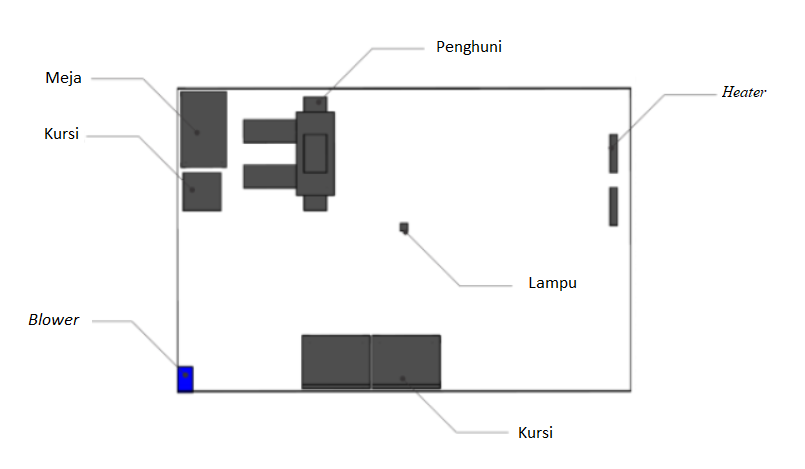
\includegraphics[width=1\textwidth]{figures/KondisiChamber}
	\caption{Posisi Komponen \textit{Climate Chamber}}
	\label{fig:5:KondisiChamber}
\end{figure}

\textit{Climate chamber} memiliki ukuran $3m \times 2m \times 3m$ ($p \times l \times t$). Komponen-komponen di dalam \textit{climate chamber} terdiri dari meja, kursi, \textit{blower}, penghuni, lampu, \textit{heater}, dan AC. 

\begin{figure}[h]
	\centering
	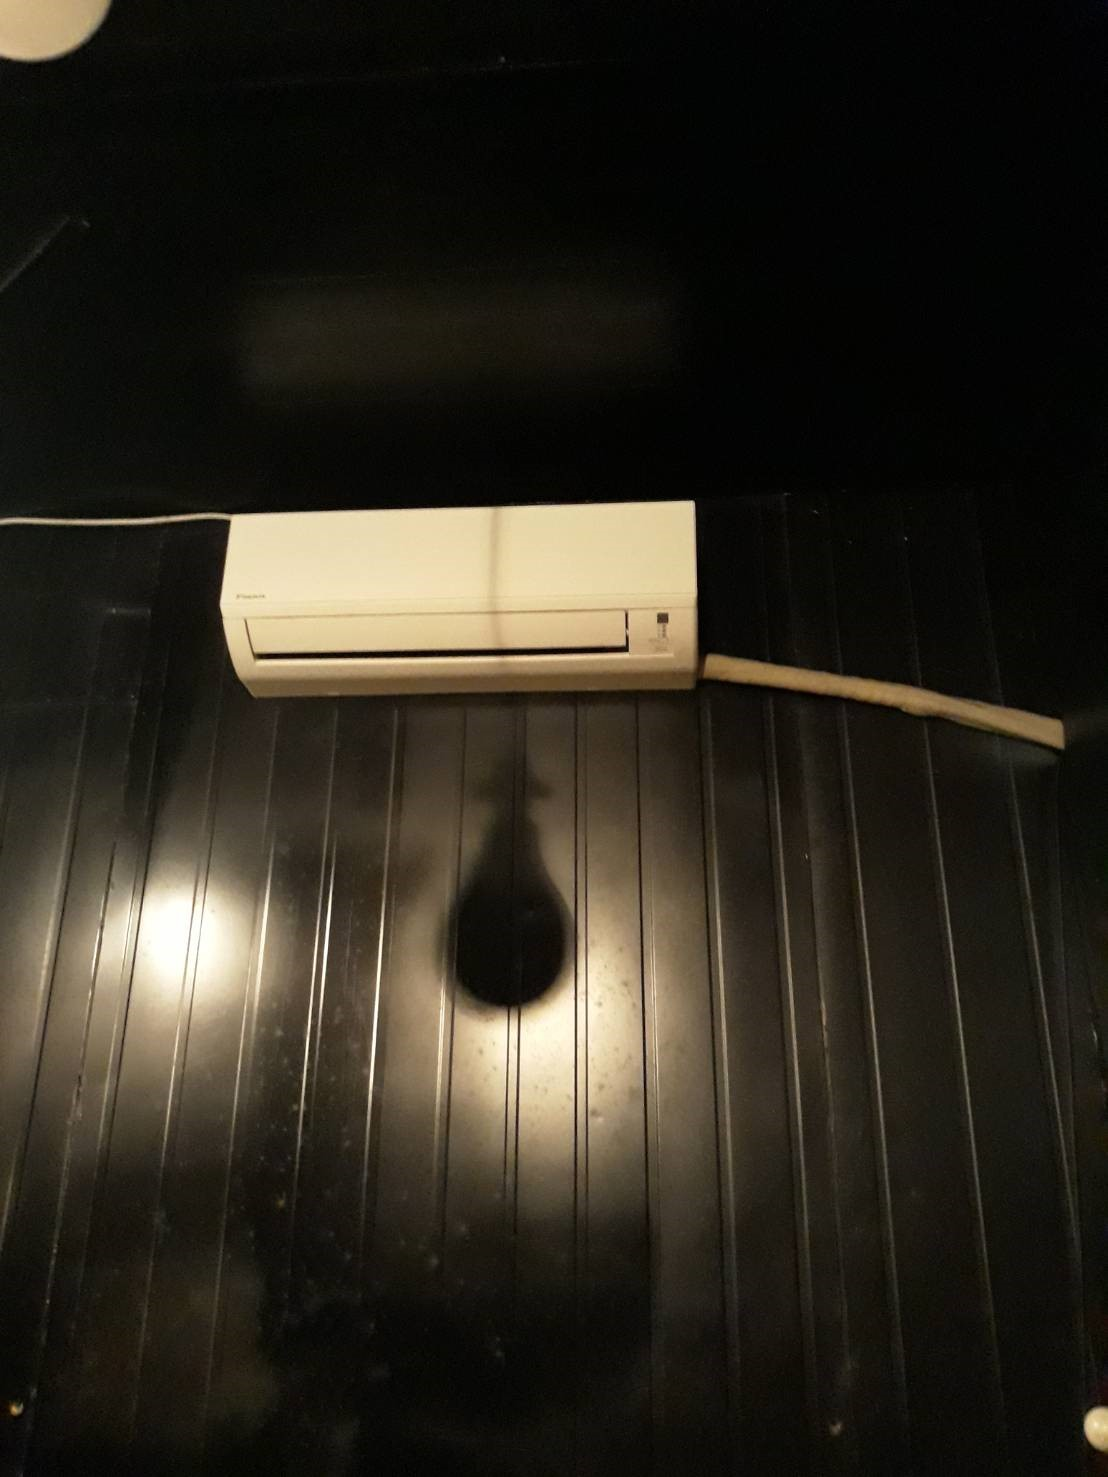
\includegraphics[width=0.8\textwidth]{figures/AC}
	\caption{Perangkat AC}
	\label{fig:5:AC}
\end{figure}

\begin{figure}[!h]
	\centering
	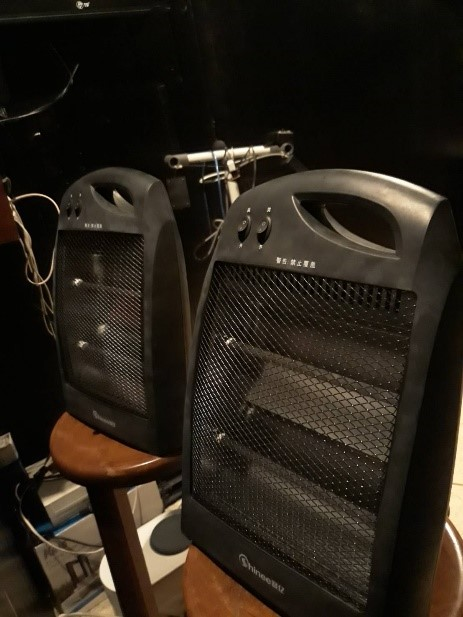
\includegraphics[width=0.5\textwidth]{figures/Heater}
	\caption{Perangkat \textit{Heater}}
	\label{fig:5:Heater}
\end{figure}	

Perangkat AC yang berada di dalam \textit{climate Chamber} DTNTF UGM memiliki daya sebesar 2800W (1 PK). Perangkat AC mampu mengkondisikan lingkungan melalui aliran udara yang keluar. Maka dari itu, Perangkat AC sangatlah berpengaruh terhadap kondisi lingkungan termal di dalam ruangan. Tampak dari wujud perangkat AC dapat dilihat pada Gambar \ref{fig:5:AC}.

Perangkat \textit{heater} yang berada di dalam \textit{climate chamber} memiliki daya sebesar 900W. Terdapat dua buah perangkat \textit{heater} di dalam \textit{climate chamber}. Semakin banyak perangkat heater yang aktif maka akan suhu udara akan menjadi semakin meningkat. Kenaikan rerata suhu udara yaitu sebesar $\pm$1,9$^{\circ}$C untuk setiap perangkat \textit{heater}. Tampak dari wujud perangkat \textit{heater} dapat dilihat pada Gambar \ref{fig:5:Heater}.

Selain faktor dari dalam \textit{climate chamber}, faktor dari luar ruangan \textit{climate chamber} pun secara tidak langsung mempengaruhi kondisi lingkungan termal \textit{climate chamber}. Diantaranya adalah suhu udara luar (\textit{dry bulb temperature}) dan intensitas radiasi matahari. Posisi harian matahari mempengaruhi perubahan nilai suhu udara luar dan intensitas radiasi matahari. Pada siang hari (posisi \textit{altitude} matahari ketika berada tepat diatas \textit{climate chamber}) akan memberikan paparan radiasi matahari yang mengenai selubung bangunan dan menaikkan suhu udara luar. Hal ini menyebabkan suhu di dalam \textit{climate chamber} naik. Kalor yang menembus pada selubung bangunan akan sebanding dengan nilai U-value. Nilai U-Value pada selubung bangunan dapat dilihat pada Tabel \ref{tbl:5:UValue}.

\begin{table}[hbt!]
	\caption{U-Value Selubung \textit{Climate Chamber}}
	\label{tbl:5:UValue}
	\centering
	% use packages: array
	\begin{tabular}{|l|l|}
		\hline
		\textbf{Selubung \textit{climate chamber}} & \textbf{U-Value (W/m$^2$.K)} \\ \hline
		Dinding & 0,707 \\ \hline
		Lantai  & 1,996 \\ \hline
		Atap    & 0,707 \\ \hline
	\end{tabular}
\end{table}

\subsection{Hasil Rancangan Skenario}
Rancangan skenario pada \textit{climate chamber} menghasilkan kombinasi antara set AC dan jumlah \textit{heater} ON. Set AC dikondisikan untuk menyala dari pukul 08:00 s.d. 17:00 dengan rentang nilai 16$^\circ$C - 30$^\circ$C. Set jumlah \textit{heater} ON terbagi menjadi 3 kondisi, yaitu keduanya tidak menyala (berkode 0), salah satu menyala (berkode 1), dan keduanya menyala (berkode 2). Kombinasi tersebut menghasilkan 25 variasi skenario. Untuk variasi suhu luar dan intensitas radiasi matahari, penulis bersama Tanto sepakat untuk menggunakan 4 titik ekstrim bumi terhadap matahari yaitu pada tanggal 21 Maret, 21 Juni, 23 September dan 22 Desember. Kemudian kami melakukan simulasi disetiap titik tersebut dengan kombinasi set \textit{heater} dan set AC seperti pada Gambar \ref{fig:5:HeaterAC}. Sehingga, total skenario yang dihasilkan dari kombinasi tersebut berjumlah 100 skenario.
\begin{figure}[!h]
	\centering
	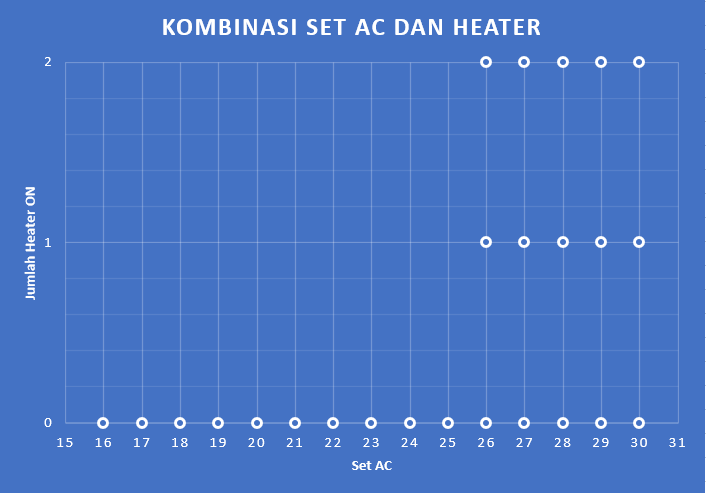
\includegraphics[width=0.8\textwidth]{figures/HeaterAC}
	\caption{Skenario Set Suhu AC dan Jumlah Heater ON}
	\label{fig:5:HeaterAC}
\end{figure}


\subsection{Hasil Simulasi IES-VE}

\section{Pembangunan Arsitektur JST}
Data dibagi menjadi 3 bagian, yakni 70\% data pelatihan, 15\% data validasi, dan 15\% data pengujian. Model JST menggunakan arsitektur \textit{multilayer perceptron} dengan jumlah neuron sebanyak $x_1$ di lapisan tersembunyi 1, $x_2$ di lapisan tersembunyi 2, dan $x_3$ di lapisan tersembunyi 3.

\section{Analisis Kinerja Arsitektur JST yang terpilih}

Persamaan ditulis rata tengah dan nomor persamaan ditulis rata kanan. Nomor persamaan
diurutkan dengan format (nomor\_bab.nomor\_persamaan). Contoh dapat dilihat pada Persamaan \eqref{eq:1}.

\begin{equation}
    \dfrac{Dv}{Dt} = \dfrac{\partial v}{\partial t} + \nabla \cdot \mathbf{uu}
\label{eq:1}
\end{equation}

